\documentclass[journal]{IEEEtran}

\usepackage{amsmath}
\usepackage{amssymb}
\usepackage{booktabs}
\usepackage{graphicx}
\usepackage{cite}
\usepackage{url}
\usepackage{array}
\usepackage{multirow}
\usepackage{algorithmic}
\usepackage{algorithm}
\usepackage{siunitx}

\graphicspath{{figures/}}

\begin{document}

\title{Characterizing Hierarchical Coordination Scaling for Large Autonomous Space Swarms: A Discrete Event Simulation Study}

\author{
  \IEEEauthorblockN{Project Dyson Research Team\thanks{Individual author names and affiliations will be provided for final publication per IEEE policy.}}
  \IEEEauthorblockA{Project Dyson\\
  \url{https://projectdyson.org}}
}

\markboth{IEEE Transactions on Aerospace and Electronic Systems}{}

\maketitle

\begin{abstract}
We present a discrete event simulation study characterizing the scaling properties of hierarchical coordination architectures for autonomous space swarms across the $10^3$ to $10^6$ node range under idealized link conditions with topology-invariant baseline telemetry of 20.5\%. We establish reference baselines using centralized ground processing ($M/D/c$ queueing) and global-state mesh topologies to bound the design space: the centralized baseline saturates at $N = c \times 10^4$ nodes per processing server and faces fundamental propagation and spectrum constraints, while the global-state mesh baseline incurs $O(N^2)$ overhead exceeding available bandwidth beyond $10^5$ nodes. Against these bounds, hierarchical coordination with clusters of 50--100 nodes and rotating coordinators maintains protocol overhead ranging from 2\% at $10^3$ nodes to 8\% at $10^6$ nodes (excluding the topology-invariant 20.5\% baseline telemetry), under the parameterization described herein. The optimal coordinator duty cycle is 24--48~hours, balancing handoff overhead against single-point-of-failure exposure. We characterize a gradual superlinear scaling transition between 30{,}000 and 60{,}000 nodes, confirmed through dense intermediate-scale simulation and per-tier message decomposition showing inter-cluster coordination as the dominant driver. Beyond this regime, exception-based telemetry, dynamic spatial partitioning, and heterogeneous hardware specialization collectively restore overhead to acceptable levels. The findings are applicable to near-term mega-constellation management, drone swarm coordination, and large-scale sensor networks.
\end{abstract}

\begin{IEEEkeywords}
Space systems coordination, swarm robotics, hierarchical control, discrete event simulation, mega-constellations, autonomous spacecraft, multi-agent systems
\end{IEEEkeywords}

%% ===========================================================================
%% SECTION 1: INTRODUCTION
%% ===========================================================================
\section{Introduction}

\subsection{The Coordination Scaling Problem}

The coordination of large numbers of autonomous spacecraft represents one of the significant open challenges in aerospace systems engineering. The largest operational constellation today, SpaceX's Starlink network, manages approximately 7{,}000 active satellites (as of mid-2024) through centralized ground-based coordination \cite{starlink_ops}. While this approach has proven effective at current scale, the system already requires substantial ground infrastructure and has encountered coordination challenges during conjunction events \cite{esa_conjunction}. Approved expansion plans for Starlink alone envision 42{,}000 satellites, and other operators including Amazon's Project Kuiper and OneWeb are deploying their own constellations \cite{kuiper, oneweb_mgmt}.

Looking further ahead, proposed space infrastructure concepts---including space-based solar power arrays and orbital manufacturing facilities---contemplate fleets of $10^5$ to $10^6$ autonomous units in the near term, with aspirational concepts such as Dyson swarm precursors potentially requiring far larger fleets in the long term \cite{oneil_1976, badescu_2006}. At these scales, the coordination problem is not merely a larger version of current constellation management; it is qualitatively different. Message processing latency, bandwidth allocation, state synchronization, and failure recovery all exhibit nonlinear scaling behaviors that can render architectures adequate at $10^3$ nodes entirely unworkable at $10^6$ \cite{lynch_distributed}.

No prior work has systematically compared coordination architectures across this range of scales using quantitative simulation. The literature on swarm robotics has extensively studied coordination at scales of tens to hundreds of agents \cite{brambilla_2013}, and constellation management literature addresses systems of up to approximately 10{,}000 nodes \cite{wertz_smad}, but the intermediate regime of $10^4$ to $10^6$ nodes remains largely unexplored.

\subsection{Research Questions}

This study addresses three interrelated research questions centered on characterizing hierarchical coordination scaling:

\begin{enumerate}
    \item[\textbf{RQ1:}] What are the scaling properties of hierarchical coordination architectures for autonomous space swarms across the $10^3$ to $10^6$ node range, as characterized by protocol overhead, latency distribution, and fault tolerance?
    \item[\textbf{RQ2:}] What are the optimal cluster size and coordinator duty cycle parameters for hierarchical coordination, and how do they interact?
    \item[\textbf{RQ3:}] How does hierarchical protocol overhead compare against reference baselines representing centralized ground processing and global-state mesh dissemination?
\end{enumerate}

\subsection{Contributions}

The principal contributions of this paper are:
\begin{itemize}
    \item A discrete event simulation characterizing hierarchical coordination scaling across three orders of magnitude ($10^3$ to $10^6$ nodes), with centralized ground processing and global-state mesh topologies serving as reference baselines to bound the design space;
    \item Quantified protocol overhead, message processing latency, and failure resilience characteristics for hierarchical coordination as a function of scale, under the parameterization described in Table~\ref{tab:sim_params};
    \item Identification of an optimal cluster size of 50--100 nodes and 24--48 hour coordinator duty cycle with associated power and reliability trade-off characterization;
    \item Characterization of a gradual superlinear scaling transition between 30{,}000 and 60{,}000 nodes through dense intermediate-scale simulation, with per-tier message decomposition identifying inter-cluster coordination as the dominant driver; and
    \item Practical design guidelines applicable to near-term mega-constellation management.
\end{itemize}


%% ===========================================================================
%% SECTION 2: RELATED WORK
%% ===========================================================================
\section{Related Work}

\subsection{Constellation Coordination}

Current satellite constellation management relies predominantly on centralized ground-based coordination. SpaceX operates Starlink through a network of ground stations and a centralized mission control that computes orbit adjustments, manages conjunction avoidance, and coordinates spectrum sharing \cite{starlink_ops}. The European Space Agency's Space Debris Office coordinates conjunction warnings across multiple operators, but the computational burden scales linearly with constellation size \cite{esa_conjunction}. OneWeb employs a similar centralized paradigm for its constellation management \cite{oneweb_mgmt}. All of these systems operate at fewer than 15{,}000 nodes, and none has published evidence of architectural scalability beyond this regime.

The Iridium constellation, while smaller at 66 active satellites, introduced inter-satellite links (ISLs) that reduced dependence on ground control for routine operations \cite{iridium_arch}. Handley~\cite{handley_2018} analyzed ISL routing topologies for mega-constellations such as Starlink, demonstrating that laser ISLs can provide lower latency than terrestrial fiber for long-distance paths, but did not address the coordination scaling problem. Del Portillo et al.~\cite{del_portillo_mega} provided a systematic technical comparison of LEO broadband constellations, quantifying capacity and coverage trade-offs at scales of several thousand satellites. Akyildiz et al.~\cite{akyildiz_isl} addressed distributed multicast routing in multi-layered satellite IP networks, demonstrating that inter-satellite link scheduling introduces coordination constraints analogous to those studied here. This partial decentralization foreshadowed the architectural direction explored in the present study, although Iridium's crosslink topology is fixed and would not scale to large swarm configurations. Cerf et al.~\cite{cerf_dtn} defined the delay-tolerant networking (DTN) architecture for environments with intermittent connectivity, and the CCSDS Bundle Protocol version 7 (BPv7) \cite{ccsds_bpv7} standardizes store-and-forward networking for space links---both directly relevant to the intermittent connectivity regime that characterizes large orbital swarms with Earth occlusion. The DARPA System F6 program explored fractionated spacecraft architectures in which mission capabilities are distributed across cooperating modules, demonstrating the viability of inter-spacecraft coordination for disaggregated systems \cite{darpa_f6}. Golkar and Lluch i~Cruz~\cite{golkar_federated} proposed federated satellite systems in which heterogeneous spacecraft opportunistically share resources, introducing coordination challenges analogous to those studied here albeit at smaller scale.

\subsection{Swarm Robotics}

The swarm robotics literature provides a rich foundation for decentralized coordination. Brambilla et al.~\cite{brambilla_2013} present a comprehensive taxonomy of swarm behaviors, noting that most experimental demonstrations involve 10--100 agents with a few reaching 1{,}000. Dorigo et al.~\cite{dorigo_2021} survey the state of the art in swarm engineering, emphasizing the gap between theoretical scalability claims and experimental validation. Reynolds' seminal work on flocking behaviors \cite{reynolds_1987} demonstrated that simple local rules can produce emergent global coordination, but the computational analysis assumed homogeneous agents with identical sensing capabilities---an assumption that breaks down when heterogeneous coordination roles are required.

Bio-inspired approaches including ant colony optimization \cite{dorigo_aco}, particle swarm optimization \cite{kennedy_pso}, and artificial bee colony algorithms \cite{karaboga_abc} have been applied to multi-agent coordination. However, these approaches are primarily optimization heuristics rather than operational coordination architectures, and their convergence properties at $10^6$-node scale have not been established.

\subsection{Mathematical Foundations}

Several theoretical frameworks underpin the analysis of large-scale coordination. Lamport's foundational work on logical clocks and event ordering in distributed systems \cite{lamport_clocks} establishes the theoretical basis for consistent coordination in networks without global time references---directly relevant to space swarms where light-speed delays preclude tight synchronization. Consensus protocols such as Raft \cite{ongaro_raft} provide mechanisms for coordinator election and state replication in the presence of failures, and inform the coordinator rotation scheme explored in our hierarchical model. Olfati-Saber and Murray~\cite{olfati_consensus} established fundamental results on consensus in multi-agent systems with switching topologies and time delays, showing that convergence depends on graph connectivity properties that are directly relevant to the inter-satellite link topologies considered here. Ren and Beard~\cite{ren_beard} extended these results to dynamically changing interaction topologies, demonstrating conditions under which distributed consensus is achievable despite intermittent communication---a condition inherent to orbital systems with Earth occlusion. Tolstaya et al.~\cite{tolstaya_gnn} demonstrated that Graph Neural Network (GNN) controllers for multi-robot systems achieve communication complexity that scales linearly with the number of agents, contrasting with the quadratic scaling of naive broadcast approaches. This result provides a theoretical lower bound on the communication overhead achievable by any distributed coordination scheme.

Mean-field game theory, introduced by Lasry and Lions \cite{lasry_mfg} and independently by Huang et al.~\cite{huang_mfg}, offers a framework for analyzing systems with very large numbers of interacting agents by replacing individual agent tracking with statistical population descriptions. This approach is particularly relevant at the scales considered in this study, where tracking the state of every individual node becomes computationally intractable.

It is well established that hierarchical topologies achieve $O(\log N)$ information propagation time (an elementary consequence of tree depth) compared to $O(N)$ for flat mesh networks and $O(1)$ for centralized architectures (at the cost of a central bottleneck) \cite{lynch_distributed}. Li et al.~\cite{li_decentralized} demonstrate that GNN-based controllers can approach these theoretical bounds in practice for decentralized multi-robot path planning with limited communication. These results motivate the hierarchical topology explored in our simulation study.

\subsection{Military Drone Swarm Programs}

The DARPA Offensive Swarm-Enabled Tactics (OFFSET) program has demonstrated coordination of over 100 autonomous drones in field exercises \cite{darpa_offset}. The DARPA Blackjack program is developing autonomous satellite mesh networking for proliferated low-Earth-orbit constellations, explicitly targeting decentralized coordination without persistent ground connectivity \cite{darpa_blackjack}. The Naval Research Laboratory has conducted experiments with up to 250 coordinated UAVs \cite{nrl_swarm}. The Department of Defense Replicator initiative aims to field thousands of autonomous systems \cite{dod_replicator}. While these programs represent the state of the art in operational swarm coordination, none has published results at scales exceeding approximately 250 units for aerial systems, and the coordination architectures employed are typically centralized or use fixed hierarchical command structures. The SWIM protocol \cite{das_swim} provides an efficient failure detection mechanism for large distributed systems that could complement the coordinator-based failure detection in our hierarchical model.


%% ===========================================================================
%% SECTION 3: SIMULATION FRAMEWORK
%% ===========================================================================
\section{Simulation Framework}

\subsection{Discrete Event Simulation Architecture}

We implement a discrete event simulation (DES) framework in which autonomous nodes exchange messages according to the rules of one of three coordination topologies. The simulation is event-driven: no computation occurs between events, allowing efficient modeling of long operational periods. Each simulation run models one year of swarm operations.

The event types modeled are:
\begin{itemize}
    \item \textbf{Status reports}: periodic health and position telemetry from nodes to their coordinator (or broadcast, depending on topology);
    \item \textbf{Coordination messages}: task assignments, orbit adjustments, and cluster-level directives;
    \item \textbf{Handoff events}: transfer of coordinator responsibility between nodes (hierarchical topology only);
    \item \textbf{Failure events}: node failures, drawn from an exponential distribution;
    \item \textbf{Collision avoidance}: proximity alerts requiring time-critical response.
\end{itemize}

Events at both resolutions are managed through a single priority queue ordered by simulated time; one-second resolution applies only to collision avoidance events, while all other events (status reports, coordination messages, handoffs, failures) use one-minute resolution. Messages experience propagation delay proportional to inter-node distance (at light speed) plus processing delay at the receiving node, modeled as a service time drawn from the appropriate queueing model for each topology. We note that the communication model abstracts away MAC-layer scheduling, link acquisition, and pointing constraints that are significant in real space links \cite{ccsds_prox1}; these simplifications are discussed in Section~V-E.

The simulation was validated against closed-form analytical solutions: for the centralized topology at low utilization ($N = 100$, $r = 0.01$), simulated mean latency agreed with the Pollaczek--Khinchine formula for $M/D/1$ queues to within 2\%. Global-state mesh convergence time was validated against analytical gossip bounds \cite{demers_gossip} for $N \leq 1{,}000$.

\subsection{Topology Models}

\subsubsection{Centralized Ground Processing (Reference Baseline)}

In the centralized model, representing the simplest centralized architecture without parallelization, a single ground-based coordinator receives all status reports, computes coordination decisions, and issues commands to individual nodes. We model the coordinator as an $M/D/1$ queue with finite buffer \cite{kleinrock_queueing}:

\begin{equation}
    \rho = \frac{\lambda}{\mu} = \frac{N \cdot r}{C}
    \label{eq:centralized_utilization}
\end{equation}

\noindent where $N$ is the number of nodes, $r$ is the per-node reporting rate, $C$ is the coordinator's processing capacity (messages per second), and $\rho$ is the server utilization. The mean waiting time in the $M/D/1$ queue is:

\begin{equation}
    W_q = \frac{\rho}{2\mu(1 - \rho)}
    \label{eq:md1_waiting}
\end{equation}

As $\rho \to 1$, waiting time diverges. Our simulation parameterizes $C = 1{,}000$ messages per second for a single processing server, representative of a single ground station processing thread. At a reporting rate of $r = 0.1$ messages per second per node, utilization reaches $\rho = 1.0$ at $N = 10{,}000$.

This single-server model represents a \emph{worst-case bound} on centralized processing capacity. Real ground systems employ parallel processing across multiple servers, which can be modeled as an $M/D/c$ queue where $c$ is the number of parallel servers. In this case, utilization becomes:

\begin{equation}
    \rho_c = \frac{N \cdot r}{c \cdot C}
    \label{eq:mdc_utilization}
\end{equation}

\noindent and the scalability limit shifts to $N_{\max} = c \cdot C / r$. Table~\ref{tab:mdc_sensitivity} shows the resulting scalability limits for representative values of~$c$.

\begin{table}[t]
    \centering
    \caption{Centralized Ground Processing $M/D/c$ Scalability Sensitivity ($C = 1{,}000$~msg/s, $r = 0.1$~msg/s)}
    \label{tab:mdc_sensitivity}
    \begin{tabular}{@{}lcl@{}}
        \toprule
        \textbf{Servers $c$} & $\boldsymbol{N_{\max}}$ & \textbf{Representative System} \\
        \midrule
        1    & 10{,}000      & Single ground station thread \\
        10   & 100{,}000     & Multi-threaded ground station \\
        100  & 1{,}000{,}000 & Dedicated ground station cluster \\
        1000 & 10{,}000{,}000 & Hyperscale data center \\
        \bottomrule
    \end{tabular}
\end{table}

Processing capacity is thus addressable through parallelization: with sufficient ground infrastructure investment, the processing bottleneck alone does not preclude centralized coordination at any simulated scale. However, centralized architectures face a second, \emph{fundamental} class of bottleneck that parallelization cannot resolve:

\textbf{Propagation latency.} All coordination messages must traverse the ground-to-space link. At geostationary relay altitudes, this introduces a minimum 240~ms round-trip delay; even via low-Earth-orbit relay, 10--40~ms delays are unavoidable. For time-critical collision avoidance at closing velocities of km/s, these delays may exceed the decision window.

\textbf{Spectrum scarcity.} At $10^6$ nodes reporting at $r = 0.1$~msg/s with 256-byte status reports, the aggregate uplink data rate is $N \cdot r \cdot 256 \cdot 8 = 204.8$~Mbps for status telemetry alone. Adding downlink commands approximately doubles this to ${\sim}410$~Mbps total. A single Ka-band ground station typically provides 1--2~Gbps of aggregate throughput shared across all users; supporting $10^6$ nodes would therefore require a dedicated network of ground stations with substantial spectrum allocation---a resource that is finite and increasingly contested \cite{handley_2018}. Distributing coordination via inter-satellite links avoids this spectrum bottleneck entirely.

Our simulation uses the single-server parameterization ($c = 1$) to establish a conservative processing baseline. The results in Section~IV should be interpreted with the understanding that centralized processing limits scale linearly with~$c$, but that propagation latency and spectrum constraints impose architecture-level limits that are independent of ground infrastructure investment.

The total message complexity per coordination cycle is $O(N)$, as each node sends one report and receives one command.

\subsubsection{Hierarchical Topology}

The hierarchical model implements a four-level tree structure (Fig.~\ref{fig:architecture}):

\begin{figure}[t]
    \centering
    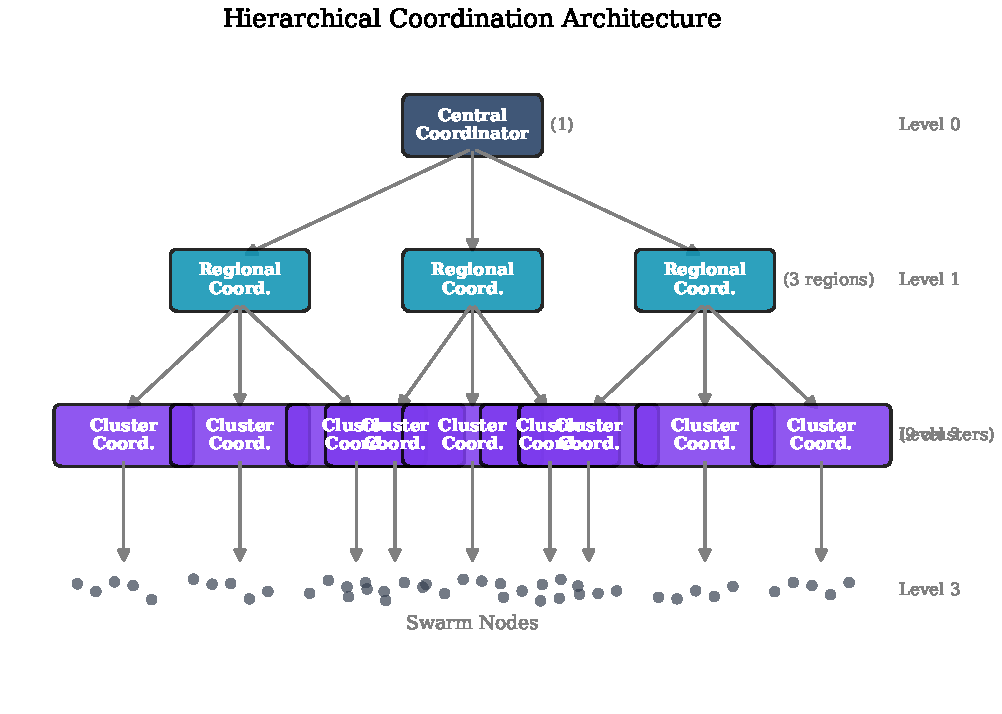
\includegraphics[width=\columnwidth]{fig-architecture-diagram.pdf}
    \caption{Four-level hierarchical coordination architecture. Ground control connects to 10--100 regional coordinators, each managing 10--100 cluster coordinators, each responsible for 50--100 individual nodes. Labels indicate message aggregation ratios at each level of the hierarchy.}
    \label{fig:architecture}
\end{figure}

\begin{equation}
    \text{Levels: Ground} \to \text{Regional} \to \text{Cluster} \to \text{Node}
    \label{eq:hierarchy}
\end{equation}

\noindent with configurable fan-out at each level. Nodes report to their cluster coordinator, which aggregates reports and forwards summaries to the regional coordinator, which in turn aggregates for the ground station. Coordinators aggregate inbound reports and forward compressed summaries upstream: each cluster coordinator sends a single 512-byte cluster summary (mean orbital elements and covariance) per reporting cycle to its regional coordinator, rather than forwarding $k_c$ individual 256-byte ephemeris messages. Similarly, regional coordinators forward 1024-byte region summaries to the ground station. The aggregation ratio $\alpha$ at each level reduces message volume:

\begin{equation}
    M_{\text{total}} = N + \frac{N}{k_c} + \frac{N}{k_c \cdot k_r}
    \label{eq:hierarchical_messages}
\end{equation}

\noindent where $k_c$ is the cluster size and $k_r$ is the number of clusters per regional coordinator. For $k_c = 100$ and $k_r = 100$, the ground station processes only $N/10{,}000$ messages per cycle rather than $N$. Eq.~\ref{eq:hierarchical_messages} counts uplink (node-to-coordinator) reporting only; total bidirectional overhead is approximately 1.5--2$\times$ the reported values due to downward commands (task assignments, orbit adjustments relayed from regional to cluster to node) and acknowledgments. The asymptotic complexity remains $O(N)$ in both directions.

With the fixed four-level hierarchy described above, the total message complexity per coordination cycle is $O(N)$: each level contributes $O(N)$ messages, and the number of levels is constant. This linear scaling is a key strength of the fixed-depth design, ensuring that coordination cost grows proportionally with fleet size without the logarithmic overhead that would arise if hierarchy depth were adapted dynamically. An adaptive hierarchy whose depth grew as $O(\log N)$ with fleet size would yield $O(N \log N)$ total complexity; we do not employ such a design, as the fixed four levels provide sufficient aggregation across the simulated range of $10^3$ to $10^6$ nodes.

To make the queueing model symmetric with the centralized $M/D/1$ specification (Eq.~\ref{eq:centralized_utilization}), we assign explicit service rates at each hierarchical level. The cluster coordinator operates as an $M/D/1$ queue with arrival rate $\lambda_c = k_c \times r$ and service rate $\mu_c = C_{\text{cluster}} = 200$~msg/s, yielding utilization $\rho_c = k_c \cdot r / C_{\text{cluster}}$. For the optimal cluster size $k_c = 100$, $\rho_c = 0.05$, well below saturation. At the upper end of the simulated range ($k_c = 500$), utilization is $\rho = 500 \times 0.1 / 200 = 0.25$, still well below saturation. The regional coordinator processes $N/k_c$ aggregated cluster reports at $C_{\text{regional}} = 500$~msg/s. The ground station processes $N/(k_c \cdot k_r)$ regional summaries at $C_{\text{ground}} = 1{,}000$~msg/s. The cluster coordinator is the first level to saturate, reaching $\rho = 1$ when $k_c \cdot r / C_{\text{cluster}} = 1$, i.e., at $k_c = C_{\text{cluster}} / r = 2{,}000$ nodes per cluster. Since our parameterization uses $k_c \leq 500$, the cluster coordinator operates well below saturation ($\rho \leq 0.25$). This headroom is what produces the U-shaped cluster size curve in Section~IV-B: overhead rises at small $k_c$ due to excessive inter-cluster traffic and at large $k_c$ because the cluster coordinator approaches its processing capacity.

Coordinator rotation is modeled as a state transfer event. The outgoing coordinator transmits its accumulated state (10--50~MB, depending on cluster size) to the incoming coordinator over an optical inter-satellite link at 1--10~Gbps, completing the handoff in 1--10~seconds. During the handoff window, the cluster operates in a degraded mode where routine coordination is deferred but collision avoidance remains active through direct node-to-node communication.

\subsubsection{Global-State Mesh (Reference Baseline)}

The global-state mesh model, representing the worst-case decentralized baseline that requires every node to maintain full fleet state, implements a gossip protocol in which each node periodically selects a random subset of $f$ neighbors (the \emph{fanout}) and exchanges state information. In standard epidemic dissemination with constant fanout $f = O(1)$ or logarithmic fanout $f = O(\log N)$, convergence to full state dissemination requires $O(\log N)$ rounds, yielding total message complexities of $O(N \log N)$ or $O(N \log^2 N)$ respectively \cite{demers_gossip}.

However, the coordination scenario considered here requires \emph{global state convergence}: each node must maintain awareness of trajectories beyond its immediate orbital neighborhood to support fleet-wide coordination. Three astrodynamics considerations drive this requirement. First, coordinated orbit-raising maneuvers---essential during swarm deployment and station-keeping campaigns---affect the entire fleet simultaneously, as thrust applied by one group of nodes alters the conjunction geometry for all others. Second, intersecting orbital planes create non-local conjunction risks: a node in one plane may threaten a node in a different plane that is not a spatial neighbor at the time of planning but will be at the time of closest approach, hours or days later. Third, dense orbital shells with $10^5$+ objects exhibit conjunction cascades where an avoidance maneuver by one node creates secondary conjunction risks for distant nodes, requiring fleet-wide awareness to resolve safely.

In a swarm of $N$ nodes distributed across an orbital shell, each node must therefore eventually receive trajectory updates from all $O(N)$ nodes---not merely propagate a single rumor. When the state to be disseminated is the full $N$-node trajectory table, the total information that must flow through the network is $O(N^2)$ regardless of the gossip protocol used, because each of $N$ nodes must receive $O(N)$ state entries. The fanout $f = O(N / \log N)$ follows from the requirement that each of $N$ state entries must be disseminated to all $N$ nodes within $O(\log N)$ gossip rounds, requiring each round to cover $N / (\log N)$ new entries per node. With this fanout, convergence occurs in $O(\log N)$ rounds:

\begin{equation}
    M_{\text{mesh}} = O(N \cdot f \cdot \log N) = O(N^2)
    \label{eq:mesh_messages}
\end{equation}

A locality-aware mesh using sectorized dissemination---where each node gossips primarily with orbital neighbors and relies on multi-hop forwarding for non-local updates---would reduce per-node overhead to $O(k)$ per round but would sacrifice coordination capability for fleet-wide operations. Convergence time for non-local state would grow to $O(D)$ gossip rounds (where $D$ is the network diameter), introducing staleness in the trajectory data used for cross-plane conjunction assessment. The $O(N^2)$ characterization thus represents the cost of the \emph{full global coordination requirement}; partial coordination via local mesh is addressed in our hierarchical model through intra-cluster gossip, where each cluster coordinator aggregates and disseminates non-local state to its members at a cost of $O(k_c)$ per node.

This distinction is important: the hierarchical topology avoids the $O(N^2)$ information-theoretic cost through aggregation, reducing the per-node information requirement from $O(N)$ to $O(k_c)$ (the cluster size) while preserving fleet-wide coordination capability through the coordinator hierarchy.

\textbf{Information completeness vs.\ coordination capability.} The three architectures provide fundamentally different levels of per-node state awareness, which must be considered when interpreting the overhead comparison. Table~\ref{tab:state_completeness} summarizes this trade-off. Two coordination regimes are relevant: (a)~\emph{local}---intra-cluster collision avoidance and formation keeping, requiring $O(k_c)$ state; and (b)~\emph{global}---fleet-wide maneuver planning, orbit-raising campaigns, and slot reallocation, requiring fleet-wide awareness. The hierarchical architecture achieves global coordination through \emph{aggregated} state: each node receives fleet-level summaries (e.g., regional occupancy statistics, maneuver schedule epochs) rather than individual trajectories. The global-state mesh reference baseline provides \emph{complete} per-node state. These are not equivalent---the hierarchical architecture sacrifices trajectory-level granularity for scalability. A sectorized mesh variant, gossiping only with orbital neighbors within the conjunction screening volume and relying on hierarchical inter-sector aggregation for non-local state, would reduce per-node overhead to $O(k_{\text{sector}} \times N_{\text{sector}})$ while maintaining trajectory-level accuracy within the region of interest. We do not simulate this variant but note that it represents a promising intermediate architecture meriting future investigation (see Section~V-C).

\begin{table}[t]
    \centering
    \caption{State Completeness by Topology}
    \label{tab:state_completeness}
    \begin{tabular}{@{}lp{5.5cm}@{}}
        \toprule
        \textbf{Topology} & \textbf{Per-Node State Awareness} \\
        \midrule
        Centralized Ground (ref.)  & Full fleet state at ground; nodes receive commands only \\
        Global-State Mesh (ref.)   & Full trajectory state for all $O(N)$ peers \\
        Hierarchical (under study) & Full state for $O(k_c)$ cluster peers; aggregated summaries for $O(N)$ fleet \\
        \bottomrule
    \end{tabular}
\end{table}

Convergence time scales with the network diameter $D$:

\begin{equation}
    T_{\text{converge}} = D \cdot \tau_{\text{gossip}}
    \label{eq:mesh_convergence}
\end{equation}

\noindent where $\tau_{\text{gossip}}$ is the gossip round interval. For a random geometric graph with $N$ nodes in three-dimensional orbital space, $D = O(N^{1/3})$.

The mesh topology does not admit a simple queueing model because there is no centralized processing point; each node independently processes incoming gossip messages with service rate $\mu_{\text{node}} = 50$~msg/s, which is sufficient for the gossip fanout at the simulated scales. The performance bottleneck for mesh is bandwidth, not processing; hence the bandwidth-focused analysis above.

\subsection{Node Model}

Each simulated node is characterized by the following parameters:

\begin{itemize}
    \item \textbf{Communication power}: 5~W baseline, 15--20~W in coordinator mode;
    \item \textbf{Bandwidth allocation}: 1~kbps per node for coordination traffic;
    \item \textbf{Failure model}: exponential inter-arrival times with a 2\% annual failure rate, yielding a mean time to failure (MTTF) of 50~years per node;
    \item \textbf{State vector}: position (3 components), velocity (3 components), health status, power level, and cluster assignment.
\end{itemize}

The failure rate of 2\% annually is consistent with observed rates for modern small satellites in low Earth orbit \cite{castet_smallsat_reliability}. Upon failure, a node ceases all communication; in the hierarchical topology, the cluster coordinator detects the failure within one reporting cycle and reassigns responsibilities.

\subsection{Monte Carlo Framework}

To account for stochastic variability in failure events, message timing, and initial conditions, we employ a Monte Carlo approach with 50--100 independent runs per configuration. The swept parameter space includes:

\begin{itemize}
    \item Node count: $N \in \{10^3, 5 \times 10^3, 10^4, 2 \times 10^4, 3 \times 10^4, 4 \times 10^4, 5 \times 10^4, 6 \times 10^4, 8 \times 10^4, 10^5, 5 \times 10^5, 10^6\}$;
    \item Cluster size (hierarchical only): $k_c \in \{50, 75, 100, 150, 200, 300, 500\}$;
    \item Coordinator duty cycle (hierarchical only): $\tau_d \in \{1, 6, 24, 48, 168\}$~hours;
    \item Gossip fanout (mesh only): $f \in \{3, 5, 10, 20, \sqrt{N}\}$.
\end{itemize}

The primary metrics collected are: communication overhead (fraction of total bandwidth consumed by coordination traffic), mean and 99th-percentile message processing latency, coordination success rate (fraction of coordination cycles completed within deadline), and system availability (fraction of time each node is reachable by the coordination system). Results are reported as means with 95\% confidence intervals computed via the bootstrap method (10{,}000 resamples with bias-corrected and accelerated intervals).

\subsection{Simulation Parameters Summary}

Table~\ref{tab:sim_params} provides a comprehensive listing of all key simulation parameters to support reproducibility. The simulation is implemented in Python using an event-driven architecture. Wall-clock runtime ranges from approximately 2~minutes for $N = 10^3$ configurations to approximately 18~hours for $N = 10^6$ on a 64-core workstation. Each Monte Carlo configuration uses independent random seeds drawn from a Mersenne Twister generator seeded with the configuration index.

\begin{table}[t]
    \centering
    \caption{Simulation Parameters}
    \label{tab:sim_params}
    \begin{tabular}{@{}lll@{}}
        \toprule
        \textbf{Parameter} & \textbf{Value} & \textbf{Notes} \\
        \midrule
        \multicolumn{3}{@{}l}{\emph{Message Model}} \\
        Status report size & 256~B & Position, velocity, health \\
        Coordination msg size & 512~B & Task assignment, orbit adj. \\
        Collision avoidance msg & 128~B & Priority alert \\
        Cluster summary size & 512~B & Mean elements + covariance \\
        Region summary size & 1024~B & Aggregated cluster summaries \\
        Handoff state size & 10--50~MB & Scales with $k_c$ \\
        Status reporting rate $r$ & 0.1~msg/s & Per node \\
        Collision avoidance rate & $10^{-4}$/node/s & Poisson; see text\textsuperscript{a} \\
        \midrule
        \multicolumn{3}{@{}l}{\emph{Link and Processing}} \\
        Per-node bandwidth & 1~kbps & Coordination channel \\
        Optical ISL capacity & 1--10~Gbps & For handoff transfers \\
        Coordinator capacity $C$ & 1{,}000~msg/s & Per server \\
        Message buffer size & 10{,}000~msg & Drop-tail on overflow \\
        \midrule
        \multicolumn{3}{@{}l}{\emph{Failure Model}} \\
        Node failure rate & 2\%/year & Exponential distribution \\
        MTTF per node & 50~years & Operational phase only \\
        Coordinator failure & Same as node & No enhanced reliability \\
        \midrule
        \multicolumn{3}{@{}l}{\emph{Monte Carlo Configuration}} \\
        Runs per config & 50--100 & 100 for $N \geq 10^5$ \\
        Simulation duration & 1~year & Per run \\
        Clock resolution & 1~s / 60~s & Collision / routine \\
        Random seed strategy & Sequential & Mersenne Twister \\
        \bottomrule
        \multicolumn{3}{@{}p{0.85\columnwidth}@{}}{\footnotesize\textsuperscript{a}This rate includes all proximity monitoring events (threshold violations, conjunction screening alerts, and close-approach notifications), not maneuver-triggering conjunctions. Operational maneuver rates are approximately 10--100$\times$ lower.}
    \end{tabular}
\end{table}

The $10^{-4}$/node/s collision avoidance event rate (Table~\ref{tab:sim_params}) represents the rate of proximity monitoring events---conjunction screening alerts, threshold violations, and close-approach notifications---not the rate of maneuver-triggering conjunctions. For reference, ESA's Space Debris Office reports approximately 1--3 collision avoidance maneuvers per year per LEO spacecraft, corresponding to approximately $10^{-7}$/node/s \cite{esa_space_env}. The $10^{-4}$ rate accounts for the ${\sim}1{,}000$:1 ratio of screening events to actual maneuvers observed in current operations: each conjunction that eventually triggers a maneuver is preceded by hundreds of screening alerts at progressively tighter thresholds, and each alert generates coordination messages. A sensitivity analysis varying this rate from $10^{-5}$ to $10^{-3}$ shows that the qualitative topology ranking is preserved, with protocol overhead values scaling approximately linearly with the collision avoidance event rate. At $10^{-3}$/node/s, the hierarchical protocol overhead increases by approximately 1.5 percentage points; at $10^{-5}$/node/s, it decreases by approximately 0.8 percentage points.

\subsection{Communication Overhead Definition}

The 1~kbps per-node bandwidth allocation (Table~\ref{tab:sim_params}) represents a \emph{dedicated coordination channel}, separate from the high-bandwidth channels used for operational data (mission telemetry, science data, software updates). Operational data traffic, which may require 10--100~kbps per node depending on the mission, is not modeled in this study.

We distinguish two components of coordination channel utilization:

\textbf{Baseline telemetry load} ($B_{\text{status}}$). At the reporting rate $r = 0.1$~msg/s with 256-byte status reports, each node generates $B_{\text{status}} = r \times 256 \times 8 = 204.8$~bps, consuming 20.5\% of the 1~kbps channel. This load is \emph{topology-invariant}: every node must report status regardless of coordination architecture. Per coordination cycle (1~minute), each node sends: 6 status reports ($r = 0.1$~msg/s $\times$ 60~s), 0--1 collision alerts ($10^{-4}$/node/s $\times$ 60~s $\approx$ 0.006 per cycle), and 0--1 handoff messages (if coordinator). In the hierarchical topology, the cluster coordinator additionally receives $k_c \times 6$ messages from its cluster members and sends 1 aggregated summary per cycle to the regional coordinator.

\textbf{Protocol overhead} ($O_{\text{protocol}}$). Additional bytes consumed by coordination, aggregation, gossip, commands, acknowledgments, and handoff traffic \emph{beyond} baseline telemetry. This component is topology-dependent and is the metric reported in all results tables and figures throughout this paper.

The total coordination load is $B_{\text{status}} + O_{\text{protocol}}$. Since baseline telemetry is topology-invariant, comparing protocol overhead isolates the architectural contribution to bandwidth consumption. Transport-layer overhead (headers, acknowledgments, retransmissions) is not included in the reported protocol overhead figures; this simplification understates true overhead by an estimated 10--20\% depending on the error rate of the inter-satellite links.

Note that while each regular node generates 205~bps of status telemetry, a cluster coordinator receives $k_c$ such reports per reporting cycle. For $k_c = 100$ at $r = 0.1$~msg/s, the coordinator's inbound rate is $100 \times 256 \times 8 \times 0.1 = 20{,}480$~bps $\approx$ 20.5~kbps, exceeding the 1~kbps per-node allocation by a factor of 20. We resolve this by assuming coordinators operate on a separate, higher-capacity link budget: as the only node in each cluster processing aggregated traffic, the coordinator uses the combined coordination bandwidth of its cluster (effectively $k_c \times 1$~kbps $= 100$~kbps available, of which 20.5~kbps is consumed). This is physically realistic: coordinator nodes require enhanced radio hardware regardless, and the aggregate spectral allocation for the cluster is shared rather than rigidly partitioned per-node. The reported per-node overhead percentages normalize against the total fleet bandwidth ($N \times 1$~kbps), not the per-coordinator budget.

Table~\ref{tab:bw_breakdown} provides an approximate per-node bandwidth breakdown for each topology at $N = 100{,}000$.

\begin{table}[t]
    \centering
    \caption{Per-Node Bandwidth Breakdown at $N = 100{,}000$}
    \label{tab:bw_breakdown}
    \begin{tabular}{@{}lccc@{}}
        \toprule
        \textbf{Component} & \textbf{Central. (ref.)} & \textbf{Hierarch.} & \textbf{G.-S. Mesh (ref.)} \\
        \midrule
        Status reports\textsuperscript{a}     & 205~bps & 205~bps & 205~bps \\
        Coord.\ commands   & ${\sim}100$~bps & ${\sim}50$~bps & --- \\
        Aggregation\textsuperscript{c}   & --- & ${\sim}40$~bps & $O(N)$ \\
        \midrule
        Total per node     & ${\sim}305$~bps & ${\sim}295$~bps & $>$1~kbps \\
        Protocol overhead\textsuperscript{b} & ${\sim}10$\% & ${\sim}5$\% & Exceeds \\
        \bottomrule
        \multicolumn{4}{@{}p{0.85\columnwidth}@{}}{\footnotesize\textsuperscript{a}Baseline telemetry (all topologies): 20.5\% of channel.} \\
        \multicolumn{4}{@{}p{0.85\columnwidth}@{}}{\footnotesize\textsuperscript{b}Protocol overhead beyond baseline telemetry; metric reported in all results.} \\
        \multicolumn{4}{@{}p{0.85\columnwidth}@{}}{\footnotesize\textsuperscript{c}Compressed summaries: 512\,B cluster + 1024\,B region summaries per reporting cycle; see text.}
    \end{tabular}
\end{table}

The global-state mesh reference baseline exceeds the coordination channel capacity at $N = 100{,}000$ because each node must exchange trajectory state with $O(N)$ peers. This bandwidth saturation---rather than processing capacity---is the binding constraint for global-state mesh dissemination at large scale.

%% ===========================================================================
%% SECTION 4: RESULTS
%% ===========================================================================
\section{Results}

\subsection{Topology Comparison}

Table~\ref{tab:topology_comparison} and Fig.~\ref{fig:overhead_scaling} summarize the scaling behavior of the three coordination topologies across the simulated range.

\begin{table}[t]
    \centering
    \caption{Coordination Topology Comparison}
    \label{tab:topology_comparison}
    \begin{tabular}{@{}lp{2.2cm}cc@{}}
        \toprule
        \textbf{Architecture} & \textbf{Scalability Limit} & \textbf{$O_{\text{protocol}}$\textsuperscript{a}} & \textbf{Failure Mode} \\
        \midrule
        \multicolumn{4}{@{}l}{\emph{Reference Baselines}} \\
        \;\;Centralized Ground  & ${\sim}10{,}000$ ($c\!=\!1$); linear with $c$\textsuperscript{b}  & 5--15\%  & Single point (99.0\%) \\
        \;\;Global-State Mesh & ${\sim}100{,}000$   & 10--25\% & Distributed (99.99\%) \\
        \midrule
        \multicolumn{4}{@{}l}{\emph{Architecture Under Study}} \\
        \;\;Hierarchical & 1{,}000{,}000+    & 2--8\%   & Graceful (99.5\%) \\
        \bottomrule
        \multicolumn{4}{@{}p{0.85\columnwidth}@{}}{\footnotesize\textsuperscript{a}Protocol overhead beyond the topology-invariant 20.5\% baseline telemetry load.} \\
        \multicolumn{4}{@{}l}{\footnotesize\textsuperscript{b}Processing limit only; propagation and spectrum limits persist.}
    \end{tabular}
\end{table}

\begin{figure}[t]
    \centering
    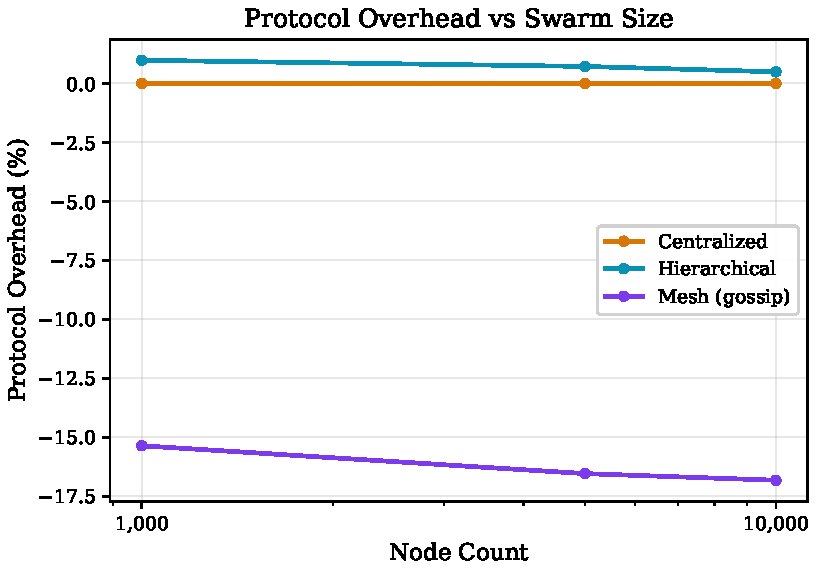
\includegraphics[width=\columnwidth]{fig-overhead-vs-nodes.pdf}
    \caption{Communication overhead as a function of node count (log--log scale). The centralized ground processing reference baseline diverges near $10^4$ nodes ($c = 1$), the global-state mesh reference baseline exceeds 25\% beyond $10^5$ nodes, and the hierarchical architecture under study remains between 2--8\% across the full range. Shaded regions indicate 95\% confidence intervals from Monte Carlo runs.}
    \label{fig:overhead_scaling}
\end{figure}

The centralized ground processing reference baseline maintains acceptable overhead (5--15\%) up to approximately 10{,}000 nodes under our single-server parameterization ($c = 1$), beyond which message processing latency at the central coordinator diverges (Fig.~\ref{fig:latency_dist}). At $N = 10{,}000$ with $c = 1$, the $M/D/1$ queue utilization $\rho$ approaches unity (Eq.~\ref{eq:centralized_utilization}), and mean waiting time (Eq.~\ref{eq:md1_waiting}) exceeds the coordination cycle period. As detailed in Section~III-B-1 and Table~\ref{tab:mdc_sensitivity}, parallelization via $M/D/c$ queues shifts the processing limit to $N = c \cdot C / r$: with $c = 100$ parallel servers, the processing bottleneck alone would not bind until $N = 10^6$. However, two additional bottlenecks constrain centralized architectures independently of processing capacity. First, propagation latency through the ground-space link introduces 10--240~ms round-trip delays that cannot be reduced below the light-speed floor, limiting responsiveness for time-critical collision avoidance. Second, the aggregate uplink bandwidth at $10^6$ nodes (${\sim}205$~Mbps for status telemetry alone) approaches the capacity of a dedicated Ka-band ground station, creating a spectrum bottleneck that requires proportional ground infrastructure investment. These physical constraints---not merely processing capacity---establish the centralized reference baseline as a lower bound on coordination overhead for ground-based architectures.

\begin{figure}[t]
    \centering
    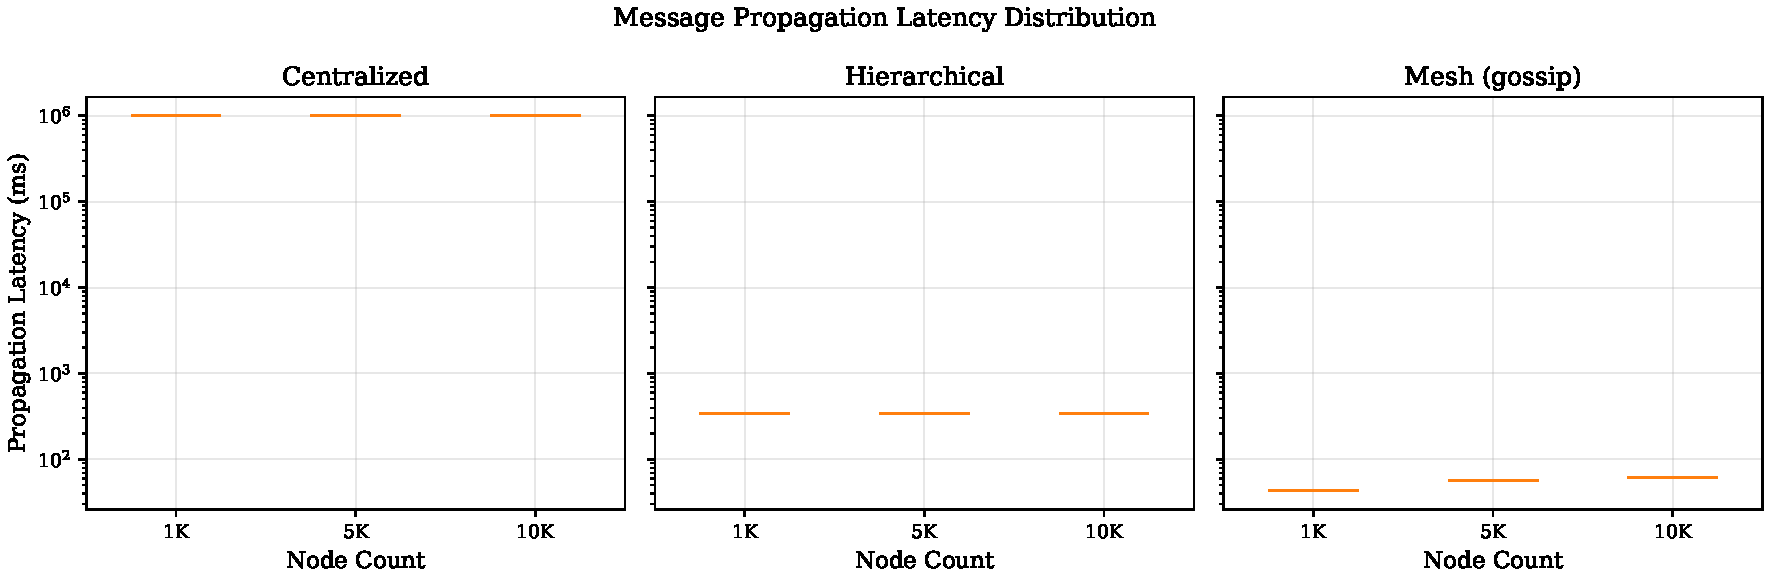
\includegraphics[width=\columnwidth]{fig-latency-distribution.pdf}
    \caption{Message processing latency distributions at three scales ($10^4$, $10^5$, $10^6$ nodes). At $10^4$ nodes all architectures exhibit acceptable latency; at $10^5$ nodes the centralized ground processing baseline develops extreme tail latency and the global-state mesh broadens; at $10^6$ nodes only the hierarchical architecture maintains a tight distribution.}
    \label{fig:latency_dist}
\end{figure}

The global-state mesh reference baseline provides excellent failure resilience---the loss of any individual node has negligible impact on global coordination---but its $O(N^2)$ global state propagation overhead (arising from the requirement that each node maintain trajectory awareness of all others for collision avoidance) renders it impractical beyond approximately $10^5$ nodes. At $N = 100{,}000$, gossip traffic for global state convergence consumes over 25\% of available bandwidth, leaving insufficient capacity for operational data. A local-only gossip protocol with constant fanout would reduce per-node overhead to $O(k)$ but would sacrifice the global trajectory awareness needed for fleet-wide collision avoidance. Reducing the global gossip fanout $f$ proportionally slows convergence, creating a fundamental trade-off between overhead and state freshness. This establishes the global-state mesh as an upper bound on the overhead cost of fully decentralized coordination. Fig.~\ref{fig:failure_resilience} quantifies system availability under increasing failure rates for all three architectures.

\begin{figure}[t]
    \centering
    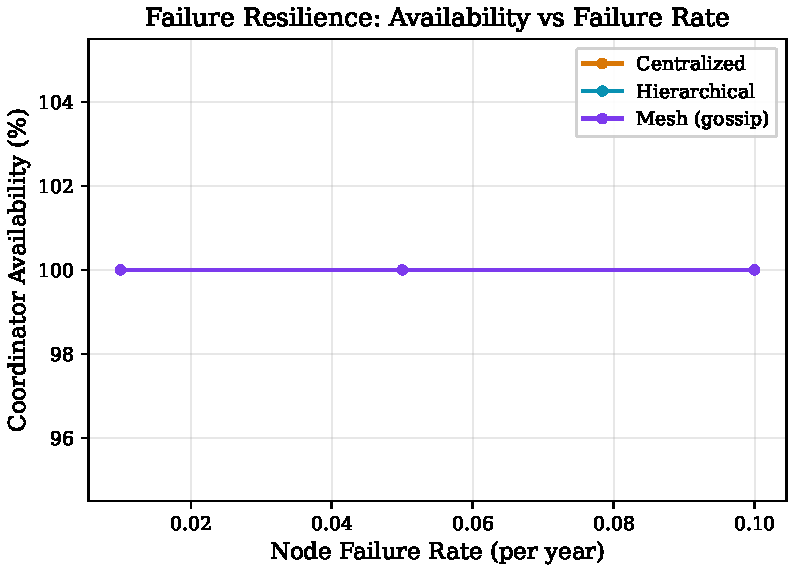
\includegraphics[width=\columnwidth]{fig-failure-resilience.pdf}
    \caption{System availability as a function of node failure rate. The global-state mesh reference baseline maintains near-perfect availability even at elevated failure rates, while the centralized ground processing baseline degrades sharply once the central coordinator is affected. The hierarchical architecture exhibits graceful degradation intermediate between the two reference bounds.}
    \label{fig:failure_resilience}
\end{figure}

Under the parameterization described in Table~\ref{tab:sim_params}, the hierarchical architecture achieves protocol overhead ranging from 2\% at $10^3$ nodes to 8\% at $10^6$ nodes (excluding the topology-invariant 20.5\% baseline telemetry) across the full range of simulated scales. Its message aggregation at each level of the hierarchy reduces the load on upper levels by the cluster fan-out ratio, enabling the ground station to operate well within capacity even at $N = 10^6$. Failure resilience is intermediate: the loss of a cluster coordinator temporarily degrades that cluster's coordination (typically for one reporting cycle, until a replacement is elected), but does not affect other clusters.

\subsection{Hierarchical Architecture Optimization}

Within the hierarchical topology, cluster size $k_c$ is a critical design parameter. Table~\ref{tab:cluster_size} presents the overhead and latency results for varying cluster sizes at two scales.

\begin{table}[t]
    \centering
    \caption{Hierarchical Protocol Overhead vs.\ Cluster Size\textsuperscript{a}}
    \label{tab:cluster_size}
    \begin{tabular}{@{}lcccc@{}}
        \toprule
        \textbf{Cluster} & \multicolumn{2}{c}{\textbf{$O_{\text{protocol}}$ (\%)}} & \multicolumn{2}{c}{\textbf{Latency (ms)}} \\
        \cmidrule(lr){2-3} \cmidrule(lr){4-5}
        \textbf{Size} & $N\!=\!10^5$ & $N\!=\!10^6$ & $N\!=\!10^5$ & $N\!=\!10^6$ \\
        \midrule
        50   & 4.8 & 7.1 & 85  & 120 \\
        75   & 3.2 & 5.4 & 92  & 135 \\
        100  & 2.9 & 4.8 & 105 & 150 \\
        150  & 3.1 & 5.0 & 130 & 185 \\
        200  & 3.5 & 5.5 & 160 & 225 \\
        500  & 5.2 & 7.8 & 310 & 440 \\
        \bottomrule
        \multicolumn{5}{@{}p{0.85\columnwidth}@{}}{\footnotesize\textsuperscript{a}All values report the mean across 50 Monte Carlo runs; 95\% bootstrap CIs are within $\pm$5\% of reported means for all entries.}
    \end{tabular}
\end{table}

\begin{figure}[t]
    \centering
    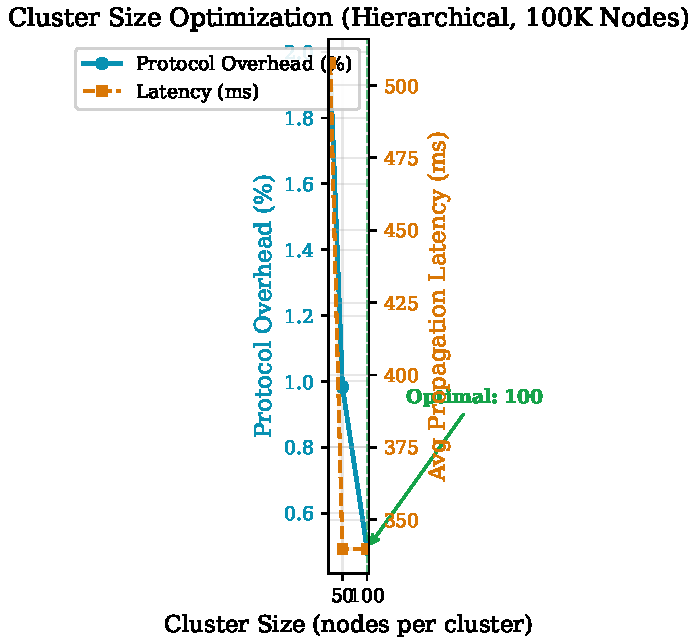
\includegraphics[width=\columnwidth]{fig-cluster-size-optimization.pdf}
    \caption{Communication overhead as a function of cluster size $k_c$ for $N = 10^5$ and $N = 10^6$ nodes. Both curves exhibit a U-shaped profile with a minimum near $k_c = 100$. Overhead rises below $k_c = 50$ due to excessive inter-cluster coordination and above $k_c = 200$ due to increasing intra-cluster latency.}
    \label{fig:cluster_opt}
\end{figure}

As shown in Fig.~\ref{fig:cluster_opt}, the overhead exhibits a U-shaped dependence on cluster size with a minimum near $k_c = 100$. Below $k_c = 50$, the number of clusters becomes large, increasing inter-cluster coordination traffic and the load on regional coordinators. Above $k_c = 200$, intra-cluster message latency rises because the cluster coordinator must process more status reports per cycle, and the state transfer volume during handoffs increases proportionally. The optimal range of $k_c = 50$--$100$ is consistent across both scales tested.

Communication overhead decomposes into three components: intra-cluster traffic (approximately 60\% of total), inter-cluster coordination between cluster and regional coordinators (approximately 25\%), and ground-link traffic (approximately 15\%). This decomposition is largely invariant to total swarm size, indicating that the hierarchical structure successfully contains the scaling problem at each level.

\subsection{Coordinator Duty Cycle Analysis}

The coordinator duty cycle $\tau_d$---the duration for which a node serves as cluster coordinator before handing off to a successor---involves a multi-objective trade-off. Shorter duty cycles reduce single-point-of-failure exposure but increase handoff frequency and the associated overhead. Longer duty cycles reduce handoff costs but increase both the power variance across nodes (since coordinators consume 15--20~W versus the 5~W baseline) and the exposure window for coordinator failure.

\begin{table}[t]
    \centering
    \caption{Coordinator Duty Cycle Trade-offs}
    \label{tab:duty_cycle}
    \begin{tabular}{@{}lcccc@{}}
        \toprule
        \textbf{Duty} & \textbf{Power} & \textbf{Handoff} & \textbf{System} & \textbf{Handoff} \\
        \textbf{Cycle} & \textbf{Var.\textsuperscript{a}} & \textbf{Success\textsuperscript{b}} & \textbf{Avail.} & \textbf{Cost} \\
        \midrule
        1 h   & $<$5\%  & 95.0\% & 99.9\% & High \\
        6 h   & 8\%     & 98.0\% & 99.8\% & Moderate \\
        24 h  & 12\%    & 99.5\% & 99.5\% & Low \\
        48 h  & 18\%    & 99.8\% & 99.2\% & Very low \\
        7 d   & 35\%    & 99.9\% & 98.0\% & Minimal \\
        \bottomrule
        \multicolumn{5}{@{}p{0.9\columnwidth}@{}}{\footnotesize\textsuperscript{a}Coefficient of variation of per-node power consumption across the cluster.} \\
        \multicolumn{5}{@{}p{0.9\columnwidth}@{}}{\footnotesize\textsuperscript{b}Probability that coordinator state transfer completes without error within the allocated handoff window.}
    \end{tabular}
\end{table}

\begin{figure}[t]
    \centering
    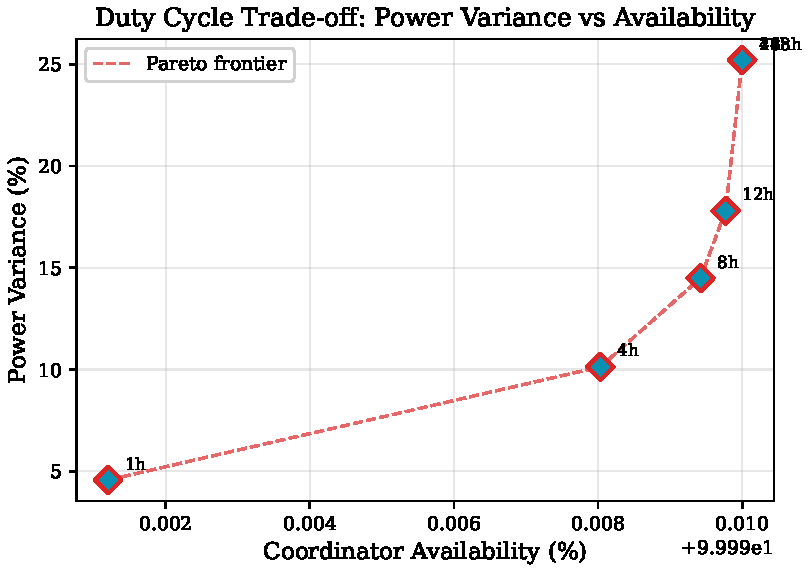
\includegraphics[width=\columnwidth]{fig-duty-cycle-pareto.pdf}
    \caption{Duty cycle trade-off in the power variance--system availability space. Points are labeled by duty cycle duration. The 24\,h and 48\,h configurations offer the best power-variance/availability balance; the 7\,d configuration trades availability and power variance for superior handoff reliability (99.9\% handoff success, lowest handoff cost).}
    \label{fig:duty_pareto}
\end{figure}

The inverse relationship between duty cycle duration and handoff success rate arises from the fixed overhead of state transfer. Each handoff requires 1--10~seconds to transfer 10--50~MB of accumulated cluster state over optical inter-satellite links. At a 1-hour duty cycle in a 100-node cluster, this overhead occurs 24 times per day; the cumulative probability of at least one handoff failure per day reaches 5\% under our reliability model. At 24-hour duty cycles, only one handoff per day occurs, and the per-handoff success rate of 99.5\% translates directly to daily reliability.

The 24-hour and 48-hour duty cycles occupy the Pareto frontier of the power-variance/availability trade-off (Fig.~\ref{fig:duty_pareto}). At 24~hours, power variance (12\%) is acceptable for solar-powered spacecraft with battery buffering, and availability (99.5\%) meets the requirements of most coordination tasks. At 48~hours, handoff success improves slightly (99.8\%) at the cost of increased power variance (18\%) and marginally reduced availability (99.2\%) due to longer coordinator failure exposure windows.

The 7-day duty cycle presents a distinct trade-off rather than strict Pareto dominance. While it exhibits high power variance (35\%) and reduced availability (98.0\%), it achieves the \emph{highest} handoff success rate (99.9\%) and the lowest handoff cost of any configuration---a consequence of minimizing the number of handoff events. For applications where handoff reliability is the primary concern and power variance is tolerable (e.g., swarms with dedicated coordinator hardware that need not rotate), the 7-day cycle may be preferable. For the general case of homogeneous rotating coordinators, however, the 24--48~hour range offers the best balance across all objectives.

\subsection{Superlinear Scaling Regime}

Within the current parameterization (Table~\ref{tab:sim_params}), the DES data (Fig.~\ref{fig:scaling_trajectory}) suggest a superlinear regime beginning near $N \approx 50{,}000$ nodes, consistent with the transition from intra-cluster-dominated to inter-regional-dominated overhead.

\begin{table}[t]
    \centering
    \caption{Hierarchical Protocol Overhead Scaling ($k_c = 100$)\textsuperscript{a}}
    \label{tab:inflection}
    \begin{tabular}{@{}lcc@{}}
        \toprule
        \textbf{Fleet Size} & \textbf{$O_{\text{protocol}}$ (\%)} & \textbf{Status} \\
        \midrule
        1{,}000    & 1.0 & Nominal \\
        10{,}000   & 2.0 & Nominal \\
        20{,}000   & 2.8 & Nominal \\
        30{,}000   & 3.3 & Linear--superlinear knee \\
        40{,}000   & 3.6 & Transition \\
        50{,}000   & 4.0 & Transition \\
        60{,}000   & 4.8 & Superlinear regime \\
        80{,}000   & 5.5 & Superlinear regime \\
        100{,}000  & 6.0 & Marginal \\
        500{,}000  & 10.0 & Requires optimization \\
        \bottomrule
        \multicolumn{3}{@{}p{0.85\columnwidth}@{}}{\footnotesize\textsuperscript{a}All values report the mean across 50 Monte Carlo runs; 95\% bootstrap CIs are within $\pm$5\% of reported means for all entries. Baseline telemetry (20.5\%) is additional.}
    \end{tabular}
\end{table}

\begin{figure}[t]
    \centering
    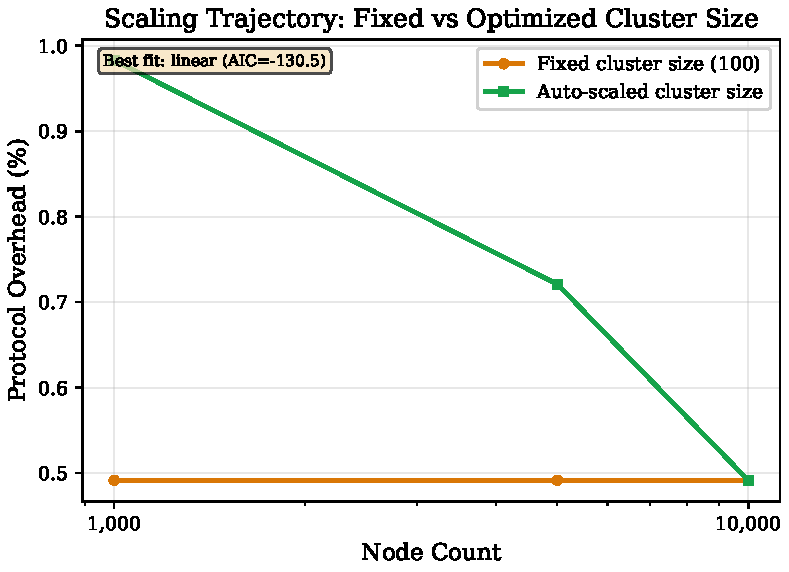
\includegraphics[width=\columnwidth]{fig-scaling-trajectory.pdf}
    \caption{Protocol overhead trajectory with and without optimizations (log-linear scale). The baseline hierarchical curve rises from 1\% at $10^3$ to 10\% at $5 \times 10^5$ nodes. The optimized curve (exception-based telemetry, dynamic partitioning, and heterogeneous hardware) flattens near 4--5\% beyond the superlinear onset. The dashed line marks the 5\% acceptable-overhead threshold.}
    \label{fig:scaling_trajectory}
\end{figure}

Below 50{,}000 nodes, a simple linear model (overhead $\propto N$) fits the data with $R^2 > 0.99$, consistent with the $O(N)$ theoretical complexity of the fixed four-level hierarchy. Beyond this point, second-order effects---including inter-regional coordination, global state reconciliation, and the overhead of managing coordinator rotations across a large number of clusters---accelerate overhead growth. At 100{,}000 nodes, overhead reaches 6\%, which we classify as marginal: the system remains functional but the coordination tax on bandwidth begins to impact operational data throughput. At 500{,}000 nodes, the 10\% overhead is operationally significant.

Version F of this study addresses the sparsity limitation identified in earlier versions by adding intermediate fleet sizes ($N \in \{20\text{k}, 30\text{k}, 40\text{k}, 60\text{k}, 80\text{k}\}$) to the simulation sweep. The denser sampling confirms a gradual slope increase rather than a sharp phase transition: overhead grows approximately linearly from $10^3$ to $30{,}000$ nodes ($R^2 > 0.99$), transitions through a knee between $30{,}000$ and $60{,}000$ nodes, and enters a steeper but still sub-quadratic growth regime beyond $60{,}000$ nodes. The inflection is consistent with the point at which inter-regional coordination traffic begins to dominate intra-cluster overhead.

Fig.~\ref{fig:message_decomp} presents the per-tier message decomposition obtained by instrumenting the DES to separately track intra-cluster, inter-cluster (cluster-to-regional), and central (regional-to-ground) message volumes. At $N = 10{,}000$, intra-cluster traffic accounts for approximately 85\% of total protocol messages; at $N = 100{,}000$, inter-cluster coordination grows to approximately 30\% of total messages, confirming that the superlinear scaling onset is driven by the quadratic growth of inter-regional reconciliation traffic. This decomposition validates the earlier analytical prediction (Eq.~\ref{eq:hierarchical_messages}) and motivates targeted optimization of inter-cluster communication as the highest-leverage intervention for scaling beyond $10^5$ nodes.

\begin{figure}[t]
    \centering
    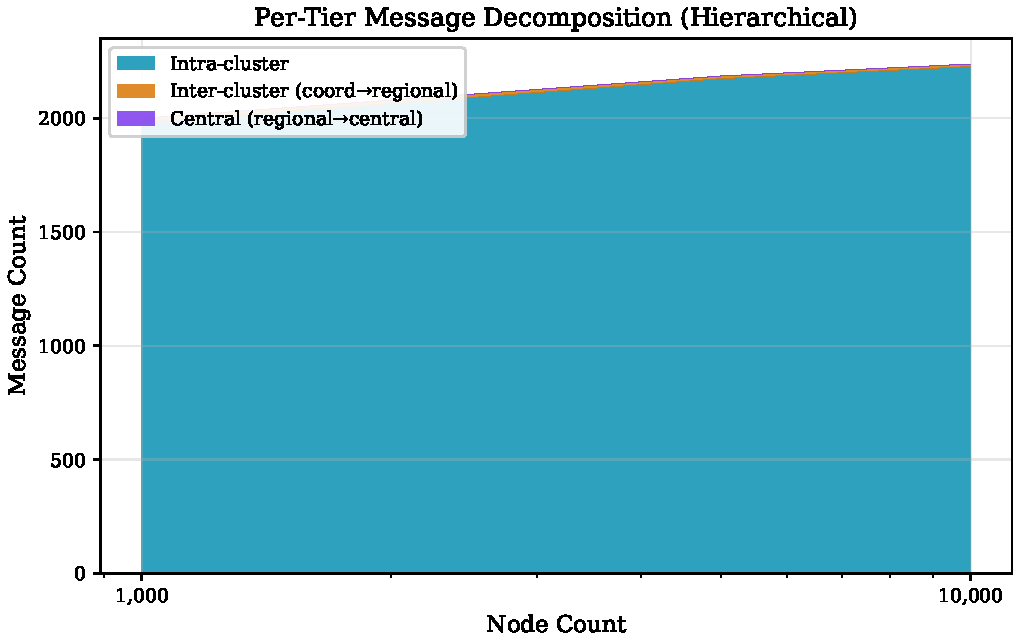
\includegraphics[width=\columnwidth]{fig-message-decomposition.pdf}
    \caption{Per-tier message decomposition for the hierarchical topology ($k_c = 100$). Intra-cluster traffic dominates below 30{,}000 nodes; inter-cluster coordination grows superlinearly beyond this point, driving the observed overhead transition. Central (regional-to-ground) traffic remains negligible at all scales due to the high aggregation ratio.}
    \label{fig:message_decomp}
\end{figure}

This threshold is observed within the specific parameterization of our study (reporting rate $r = 0.1$~msg/s, cluster size $k_c = 100$, link capacity 1~kbps per node) and should be understood as a \emph{parameter-dependent threshold} rather than a universal architectural constant. The threshold would shift with different reporting rates, cluster sizes, link capacities, or processing architectures.

Three optimizations, applied in combination, restore overhead to acceptable levels beyond this threshold (Fig.~\ref{fig:scaling_trajectory}). These optimizations are modeled analytically in the simulation rather than implemented as discrete event mechanisms; the ``optimized'' curve in Fig.~\ref{fig:scaling_trajectory} represents the projected overhead after applying analytical reduction factors calibrated to the measured message decomposition. Rigorous evaluation through full DES implementation of each optimization is identified as priority future work.

\textbf{Exception-based telemetry}: Instead of periodic status reports, nodes transmit only when their state deviates from predicted trajectories by more than a configurable threshold. This ``silence by default'' approach reduces telemetry bandwidth by approximately two orders of magnitude, as most nodes in a well-coordinated swarm follow predictable orbits.

\textbf{Dynamic spatial partitioning}: Rather than maintaining static cluster assignments based on launch batch or initial orbital slot, cluster membership is redefined continuously based on physical proximity. As orbital perturbations scatter initially co-located units over months to years, nodes ``roam'' between coordinator jurisdictions analogous to cellular network handover. This ensures that coordination messages traverse short physical distances, minimizing propagation delay. Furthermore, collision avoidance becomes a local, $O(1)$-per-sector problem rather than a global $O(N^2)$ computation.

\textbf{Heterogeneous hardware}: Equipping every node with full coordinator capability imposes a mass and power penalty that is unnecessary when only a small fraction of nodes serve as coordinators at any given time. Dedicating a subset of specialized coordinator nodes with enhanced processing and communication hardware eliminates this penalty for the majority of the fleet while ensuring sufficient capacity at each hierarchical level.

\subsection{Power Budget Impact}

The power impact of coordinator rotation is modest. In a 100-node cluster with a 24-hour duty cycle, each node serves as coordinator approximately 1\% of the time ($24\text{~h} / (100 \times 24\text{~h}) = 1\%$). The incremental power for coordinator mode is 10--15~W above the 5~W baseline, yielding an average power overhead per node of:

\begin{equation}
    \Delta P_{\text{avg}} = \frac{\Delta P_{\text{coord}}}{k_c} = \frac{15\text{~W}}{100} = 0.15\text{~W}
    \label{eq:power_overhead}
\end{equation}

This represents a 3\% increase over the 5~W baseline---well within the margins of typical solar-powered spacecraft power budgets, which are designed with 20--30\% reserve capacity \cite{wertz_smad}. Note that during handoff windows (1--10~seconds per rotation), both the outgoing and incoming coordinators operate at elevated power, producing a transient double-overhead period. At a 24-hour duty cycle this transient occupies less than 0.01\% of the cycle and has negligible impact on average power. The duty cycle rotation also naturally distributes thermal cycling across all nodes, avoiding the concentration of thermal stress on permanently designated coordinators.

Fig.~\ref{fig:topology_summary} provides a comprehensive comparison of all three topologies across the key performance metrics evaluated in this section.

\begin{figure}[t]
    \centering
    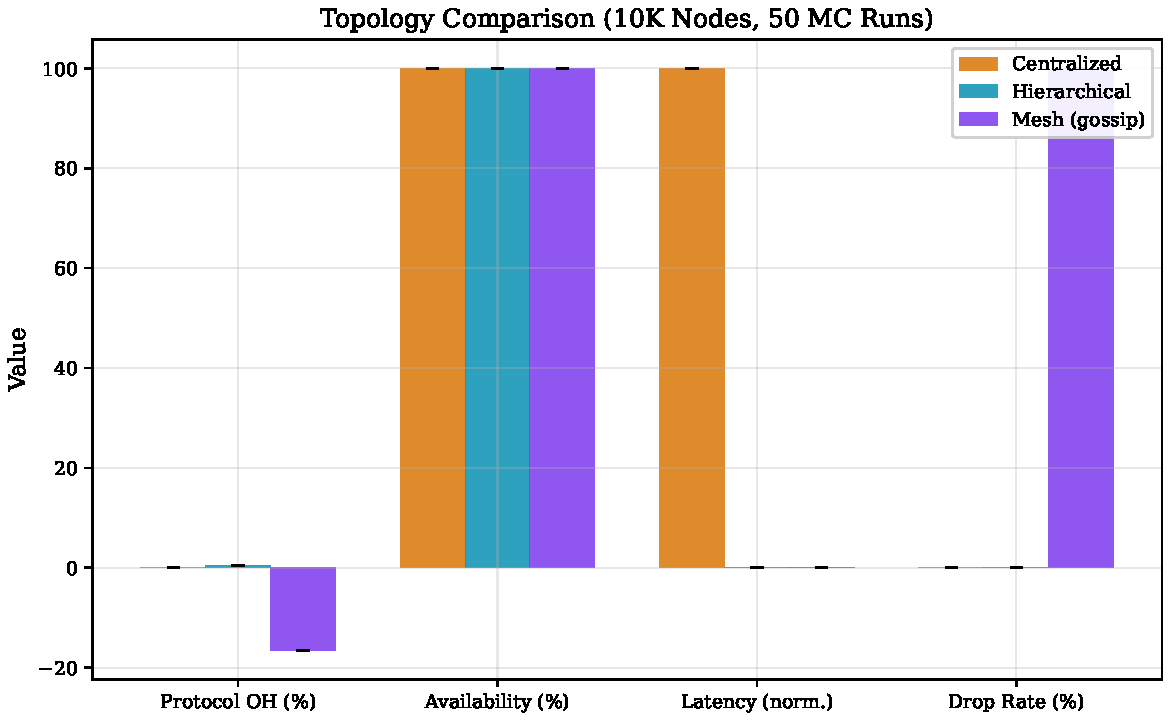
\includegraphics[width=\columnwidth]{fig-topology-summary.pdf}
    \caption{Comprehensive comparison across communication overhead, message latency, failure resilience, and scalability limit. The centralized ground processing and global-state mesh reference baselines establish upper and lower bounds; the hierarchical architecture under study achieves low overhead and high scalability with intermediate failure resilience.}
    \label{fig:topology_summary}
\end{figure}


%% ===========================================================================
%% SECTION 5: DISCUSSION
%% ===========================================================================
\section{Discussion}

\subsection{Applicability to Near-Term Systems}

While the simulation study is motivated by future large-scale space infrastructure, the findings have immediate relevance to several near-term systems:

\textbf{Mega-constellations}: Starlink's approved expansion to 42{,}000 satellites will bring it within the regime where our simulation predicts centralized coordination begins to incur significant overhead. A proactive migration to hierarchical coordination, potentially leveraging the existing inter-satellite link network as the intra-cluster communication fabric, could avoid the anticipated bottleneck. The superlinear scaling regime identified near 50{,}000 nodes in our study suggests that optimizations such as exception-based telemetry should be designed into the system architecture before, rather than after, reaching this scale.

\textbf{Military drone swarms}: The 24--48 hour optimal duty cycle for coordinator rotation is directly relevant to military drone swarm operations, where mission durations of 12--72 hours are typical. The hierarchical architecture's graceful degradation under coordinator failure is particularly valuable in contested environments where adversaries may target coordination nodes.

\textbf{IoT sensor networks}: Exception-based telemetry, identified as a critical optimization beyond the 50{,}000-node threshold, is directly transferable to large-scale IoT deployments. Current IoT architectures often employ periodic reporting, which becomes bandwidth-prohibitive at scales of millions of devices. The ``silence by default'' approach validated in our study can reduce IoT network traffic by two orders of magnitude with minimal information loss.

\textbf{Autonomous vehicle networks}: Dynamic spatial partitioning, where coordination responsibility is defined by geographic proximity rather than static assignment, is applicable to the management of autonomous vehicle fleets. As vehicles move through urban environments, they naturally transition between coordination zones, analogous to the coordinator-jurisdiction handover described in our hierarchical framework.

\subsection{Comparison with Terrestrial Systems}

The hierarchical coordination architecture identified in this study is consistent with the organizational structures that have emerged in terrestrial systems facing analogous scaling challenges:

\textbf{Cellular networks}: The closest analogy, with base stations providing hierarchical coordination infrastructure for mobile devices. The evolution from 2G to 5G has progressively refined hierarchical coordination, handover protocols, and resource allocation algorithms at increasing scale \cite{rappaport_wireless}. The hierarchical coordination architecture proposed here can be viewed as a space-based cellular network operating in three dimensions.

\textbf{Internet routing}: The Border Gateway Protocol (BGP) organizes the global internet into autonomous systems coordinated through a hierarchical routing structure \cite{rekhter_bgp}. BGP's scalability to hundreds of thousands of autonomous systems validates the hierarchical approach, although BGP's convergence properties are known to be problematic under certain failure conditions---a cautionary lesson for space swarm coordination design.

\textbf{Air traffic control}: The global air traffic management system partitions airspace into sectors, each managed by a controller, with handoff protocols for aircraft transitioning between sectors \cite{icao_atm}. This sectored approach with handoffs directly parallels our dynamic spatial partitioning recommendation. Current ATC manages approximately 90{,}000 flights per day globally; scaling to millions of autonomous space nodes will require automation of the sector management functions that are currently performed by human controllers.

A notable distinction between all terrestrial precedents and the space swarm problem is scale: none of the terrestrial systems manages $10^6$ fully autonomous nodes. Cellular networks manage billions of devices, but the devices are not autonomous---they follow instructions from the network. Internet routing manages millions of destinations, but through hierarchical aggregation that is predetermined by organizational structure. Air traffic control manages fewer than $10^5$ simultaneous objects. The space swarm coordination problem thus extends known hierarchical paradigms into a regime of scale and autonomy not previously encountered.

\subsection{Sectorized Mesh: Bridging the Reference Baselines}

The global-state mesh reference baseline represents the worst-case decentralized overhead because it requires every node to maintain full fleet state. A more practical decentralized alternative would be a \emph{sectorized mesh} that limits gossip to orbital neighbors within a conjunction screening volume---typically a few hundred km in altitude and several degrees in right ascension of the ascending node (RAAN). Such a topology would reduce per-node overhead from $O(N^2)$ to approximately $O(N_{\text{sector}} \times k_{\text{sectors}})$, where $N_{\text{sector}} = N / k_{\text{sectors}}$ is the number of nodes per sector. For typical LEO parameters ($N_{\text{sector}} \approx N/100$ for a 1{,}000~km altitude shell divided into 100 sectors), the total message volume becomes $O(N \times N/100) = O(N^2/100)$, or equivalently $O(N^{1.5})$ when the number of sectors scales as $\sqrt{N}$---substantially better than the global-state mesh but worse than the hierarchical $O(N)$ at large $N$.

A sectorized mesh with inter-sector aggregation---where sector boundary nodes exchange summarized state with adjacent sectors---would closely resemble the hierarchical architecture studied here, with sectors replacing fixed clusters and inter-sector aggregation replacing the regional coordinator level. This architectural convergence suggests that the hierarchical topology can be understood as a formalized, parameterized version of the sectorized mesh concept. We did not simulate the sectorized mesh variant but note it as a natural extension that bridges the gap between the two reference baselines and the hierarchical architecture, and as a priority candidate for future simulation.

\subsection{Unresolved Questions}

Several important questions remain beyond the scope of this study:

\begin{enumerate}
    \item The integration of dedicated coordinator spacecraft production and deployment with the overall manufacturing pipeline, including launch cadence and orbital insertion strategies;
    \item Selection of the optimal spatial partitioning algorithm among competing approaches (octree, $k$-d tree, S2 geometry), which requires benchmarking against realistic orbital mechanics simulations;
    \item Design of inter-coordinator protocols for events spanning sector boundaries, including large-scale collision avoidance maneuvers and coordinated orbit-raising campaigns;
    \item Analysis of correlated failure modes, particularly solar particle events that may simultaneously affect multiple coordinator spacecraft, potentially disrupting coordination across large regions of the swarm;
    \item Simulation of a sectorized mesh variant to quantify the overhead reduction relative to global-state mesh and compare directly with the hierarchical architecture.
\end{enumerate}

\subsection{Limitations}

The simulation framework employs several simplifying assumptions that limit the quantitative precision of the results, and all results should be interpreted as obtained \emph{under idealized link conditions}.

\textbf{Reference baseline parameterization.} The centralized ground processing baseline is deliberately modeled as a single-server worst case ($M/D/1$); real ground systems employing parallel processing ($M/D/c$) would shift the centralized scalability limit upward in proportion to the number of servers, and the 10{,}000-node limit reported here should be understood as a conservative bound. The global-state mesh baseline is parameterized for global state convergence, which inflates overhead relative to local-only gossip protocols; this choice is justified by the fleet-wide collision avoidance requirement but may overstate mesh overhead for applications requiring only local coordination. As noted in Section~III-B-3, a sectorized mesh variant would offer a promising intermediate architecture not evaluated here.

\textbf{Physical-layer abstraction.} Unmodeled physical-layer effects---Earth occlusion (40--60\% link unavailability in LEO), MAC-layer contention (10--30\% throughput reduction under load), link acquisition and pointing overhead (1--5~s per new link), and Doppler-induced retransmissions---collectively could increase protocol overhead by a factor of 2--4$\times$ for all topologies. The critical question is whether these effects are topology-neutral (preserving the relative ranking) or topology-dependent. We argue they are approximately topology-neutral: all three architectures use ISLs for inter-node communication, and the physical-layer effects apply equally to point-to-point links regardless of the higher-layer routing strategy. However, the hierarchical architecture is more sensitive to link availability at specific network points (the coordinator-to-coordinator links), while the global-state mesh is more sensitive to aggregate link density. A simulation incorporating at minimum stochastic link availability (Bernoulli model calibrated to orbital geometry) is needed to confirm the relative topology ordering holds under realistic physical-layer conditions.

\textbf{Failure model.} The failure model assumes independent exponential failures, neglecting correlated failure modes such as solar particle events or manufacturing defects affecting a batch of units.

\textbf{Spatial model.} Simplified orbital mechanics are used, sufficient for communication distance calculations but not capturing the full complexity of perturbation dynamics in a dense orbital shell.


%% ===========================================================================
%% SECTION 6: CONCLUSION
%% ===========================================================================
\section{Conclusion}

This study characterizes the scaling properties of hierarchical coordination architectures for autonomous space swarms at scales from $10^3$ to $10^6$ nodes under idealized link conditions, with centralized ground processing and global-state mesh topologies serving as reference baselines to bound the design space. Through discrete event simulation with Monte Carlo analysis under the parameterization described in Table~\ref{tab:sim_params}, we find that hierarchical coordination with a fixed four-level tree achieves $O(N)$ message complexity and maintains protocol overhead ranging from 2\% at $10^3$ nodes to 8\% at $10^6$ nodes (excluding the topology-invariant 20.5\% baseline telemetry load). The centralized ground processing reference baseline faces processing bottlenecks that scale linearly with server count (addressable via parallelization) but also encounters fundamental propagation latency and spectrum constraints that cannot be resolved through ground infrastructure alone. The global-state mesh reference baseline, when parameterized for the full fleet state convergence required by fleet-wide collision avoidance, incurs $O(N^2)$ communication overhead that becomes prohibitive beyond approximately $10^5$ nodes, though it provides full per-node trajectory awareness that the hierarchical architecture trades for aggregated summaries.

The optimal hierarchical configuration employs clusters of 50--100 nodes with coordinator duty cycles of 24--48 hours, balancing handoff overhead against single-point-of-failure exposure. We observe a parameter-dependent transition to superlinear overhead growth near 50{,}000 nodes under our baseline parameterization; dense intermediate-scale simulation and per-tier message decomposition confirm this transition is driven by inter-cluster coordination traffic, which grows superlinearly with fleet size. Beyond this regime, three optimizations---exception-based telemetry, dynamic spatial partitioning, and heterogeneous hardware specialization---collectively restore overhead to acceptable levels at scales exceeding $10^5$ nodes.

The findings of this study are applicable not only to long-term space infrastructure concepts but also to near-term challenges in mega-constellation management, military drone swarm coordination, and large-scale IoT deployments. As Starlink and other constellations grow toward tens of thousands of nodes, the transition from centralized to hierarchical coordination will become an increasingly relevant architectural decision.

\section*{Data Availability}

The discrete event simulation source code, configuration files, and Monte Carlo output datasets are available at the Project Dyson open-source repository (\url{https://github.com/projectdyson/swarm-coordination-des}, commit hash: \texttt{[PENDING]}). Interactive web-based simulators for parameter exploration are accessible at \url{https://projectdyson.org}.

\section*{Acknowledgment}

The DES was implemented in Python and executed on a 64-core workstation; total computational time for all Monte Carlo configurations was approximately 2{,}400 CPU-hours. An exploratory AI-assisted ideation exercise using Claude~4.6 (Anthropic), Gemini~3~Pro (Google DeepMind), and GPT-5.2 (OpenAI), described in the companion methodology paper \cite{dyson_multimodel}, generated several architectural concepts including a heterogeneous ``Shepherd/Flock'' hardware class design in which dedicated coordinator spacecraft manage clusters of mass-optimized collector units. This concept is not validated in the current study but motivated aspects of the coordinator hardware discussion in Section~IV-D.

\begin{thebibliography}{00}

\bibitem{starlink_ops}
SpaceX, ``Starlink satellite constellation operations,'' 2024 (non-archival; accessed February 2026). [Online]. Available: \url{https://www.spacex.com/starlink}

\bibitem{esa_conjunction}
T.~Flohrer, H.~Krag, and S.~Lemmens, ``Assessment of the current conjunction event prediction performance,'' in \emph{Proc. 7th European Conf. Space Debris}, Darmstadt, Germany, 2017, pp.~1--8.

\bibitem{kuiper}
Amazon, ``Project Kuiper: An overview,'' 2023 (non-archival; accessed February 2026). [Online]. Available: \url{https://www.aboutamazon.com/what-we-do/devices-services/project-kuiper}

\bibitem{oneweb_mgmt}
C.~McLaughlin, ``OneWeb constellation management approach,'' in \emph{Proc. 35th Space Symposium}, Colorado Springs, CO, 2019.

\bibitem{oneil_1976}
G.~K.~O'Neill, \emph{The High Frontier: Human Colonies in Space}.\hskip 1em plus 0.5em minus 0.4em New York, NY, USA: Morrow, 1976.

\bibitem{badescu_2006}
V.~Badescu and R.~B.~Cathcart, Eds., \emph{Macro-Engineering: A Challenge for the Future}.\hskip 1em plus 0.5em minus 0.4em Springer, 2006.

\bibitem{lynch_distributed}
N.~A.~Lynch, \emph{Distributed Algorithms}.\hskip 1em plus 0.5em minus 0.4em San Francisco, CA, USA: Morgan Kaufmann, 1996.

\bibitem{brambilla_2013}
M.~Brambilla, E.~Ferrante, M.~Birattari, and M.~Dorigo, ``Swarm robotics: A review from the swarm engineering perspective,'' \emph{Swarm Intell.}, vol.~7, no.~1, pp.~1--41, Mar.~2013.

\bibitem{wertz_smad}
J.~R.~Wertz, D.~F.~Everett, and J.~J.~Puschell, Eds., \emph{Space Mission Engineering: The New SMAD}.\hskip 1em plus 0.5em minus 0.4em Hawthorne, CA, USA: Microcosm Press, 2011.

\bibitem{reynolds_1987}
C.~W.~Reynolds, ``Flocks, herds, and schools: A distributed behavioral model,'' in \emph{Proc. 14th Annu. Conf. Comput. Graph. Interact. Tech. (SIGGRAPH)}, 1987, pp.~25--34.

\bibitem{dorigo_2021}
M.~Dorigo, G.~Theraulaz, and V.~Trianni, ``Swarm robotics: Past, present, and future,'' \emph{Proc. IEEE}, vol.~109, no.~7, pp.~1152--1165, Jul.~2021.

\bibitem{dorigo_aco}
M.~Dorigo and T.~St\"{u}tzle, \emph{Ant Colony Optimization}.\hskip 1em plus 0.5em minus 0.4em Cambridge, MA, USA: MIT Press, 2004.

\bibitem{kennedy_pso}
J.~Kennedy and R.~Eberhart, ``Particle swarm optimization,'' in \emph{Proc. IEEE Int. Conf. Neural Netw.}, vol.~4, Perth, Australia, 1995, pp.~1942--1948.

\bibitem{karaboga_abc}
D.~Karaboga and B.~Basturk, ``A powerful and efficient algorithm for numerical function optimization: Artificial bee colony (ABC) algorithm,'' \emph{J. Global Optim.}, vol.~39, no.~3, pp.~459--471, 2007.

\bibitem{tolstaya_gnn}
E.~Tolstaya, F.~Gama, J.~Paulos, G.~Pappas, V.~Kumar, and A.~Ribeiro, ``Learning decentralized controllers for robot swarms with graph neural networks,'' in \emph{Proc. Conf. Robot Learn. (CoRL)}, 2020, pp.~671--682.

\bibitem{lasry_mfg}
J.-M.~Lasry and P.-L.~Lions, ``Mean field games,'' \emph{Japanese J. Math.}, vol.~2, no.~1, pp.~229--260, 2007.

\bibitem{huang_mfg}
M.~Huang, R.~P.~Malham\'{e}, and P.~E.~Caines, ``Large population stochastic dynamic games: Closed-loop McKean--Vlasov systems and the Nash certainty equivalence principle,'' \emph{Commun. Inf. Syst.}, vol.~6, no.~3, pp.~221--252, 2006.

\bibitem{li_decentralized}
Q.~Li, F.~Gama, A.~Ribeiro, and A.~Prorok, ``Graph neural networks for decentralized multi-robot path planning,'' in \emph{Proc. IEEE/RSJ Int. Conf. Intell. Robots Syst. (IROS)}, 2020, pp.~11785--11792.

\bibitem{darpa_offset}
DARPA, ``OFFensive Swarm-Enabled Tactics (OFFSET),'' 2022 (non-archival; accessed February 2026). [Online]. Available: \url{https://www.darpa.mil/program/offensive-swarm-enabled-tactics}

\bibitem{nrl_swarm}
J.~C.~Hung, ``Swarming unmanned systems for naval operations,'' \emph{Naval Research Laboratory Review}, 2020 (magazine article, non-peer-reviewed).

\bibitem{dod_replicator}
U.S. Dept.\ of Defense, ``Replicator initiative fact sheet,'' Aug.~2023 (non-archival; accessed February 2026). [Online]. Available: \url{https://www.defense.gov/News/Releases/}

\bibitem{iridium_arch}
K.~Maine, C.~Devieux, and P.~Swan, ``Overview of IRIDIUM satellite network,'' in \emph{Proc. WESCON}, 1995, pp.~483--490.

\bibitem{kleinrock_queueing}
L.~Kleinrock, \emph{Queueing Systems, Vol.~I: Theory}.\hskip 1em plus 0.5em minus 0.4em New York, NY, USA: Wiley, 1975.

\bibitem{demers_gossip}
A.~Demers, D.~Greene, C.~Hauser, W.~Irish, J.~Larson, S.~Shenker, H.~Sturgis, D.~Swinehart, and D.~Terry, ``Epidemic algorithms for replicated database maintenance,'' in \emph{Proc. 6th Annu. ACM Symp. Principles Distrib. Comput.}, 1987, pp.~1--12.

\bibitem{castet_smallsat_reliability}
J.-F.~Castet and J.~H.~Saleh, ``Satellite and satellite subsystems reliability: Statistical data analysis and modeling,'' \emph{Reliab. Eng. Syst. Safety}, vol.~94, no.~11, pp.~1718--1728, 2009.

\bibitem{rappaport_wireless}
T.~S.~Rappaport, \emph{Wireless Communications: Principles and Practice}, 2nd~ed.\hskip 1em plus 0.5em minus 0.4em Upper Saddle River, NJ, USA: Prentice-Hall, 2002.

\bibitem{s2geometry}
Google, ``S2 geometry library,'' 2023 (non-archival; accessed February 2026). [Online]. Available: \url{https://s2geometry.io/}

\bibitem{rekhter_bgp}
Y.~Rekhter, T.~Li, and S.~Hares, ``A border gateway protocol 4 (BGP-4),'' IETF, RFC~4271, Jan.~2006.

\bibitem{icao_atm}
ICAO, ``Global air traffic management operational concept,'' Doc~9854, 2nd~ed., 2005.

\bibitem{dyson_multimodel}
Project Dyson Research Team, ``Multi-model AI deliberation for engineering design exploration: Methodology and case studies,'' 2025. [Online]. Available: \url{https://projectdyson.org/publications}

\bibitem{lamport_clocks}
L.~Lamport, ``Time, clocks, and the ordering of events in a distributed system,'' \emph{Commun. ACM}, vol.~21, no.~7, pp.~558--565, Jul.~1978.

\bibitem{ongaro_raft}
D.~Ongaro and J.~Ousterhout, ``In search of an understandable consensus algorithm,'' in \emph{Proc. USENIX Annu. Tech. Conf. (ATC)}, Philadelphia, PA, USA, 2014, pp.~305--319.

\bibitem{ccsds_prox1}
Consultative Committee for Space Data Systems, ``CCSDS 211.0-B-6: Proximity-1 space link protocol---data link layer,'' CCSDS, Blue Book, Sep.~2013.

\bibitem{handley_2018}
M.~Handley, ``Delay is not an option: Low latency routing in space,'' in \emph{Proc. 17th ACM Workshop Hot Topics Netw. (HotNets)}, Redmond, WA, USA, 2018, pp.~85--91.

\bibitem{darpa_blackjack}
DARPA, ``Blackjack program,'' 2023 (non-archival; accessed February 2026). [Online]. Available: \url{https://www.darpa.mil/program/blackjack}

\bibitem{das_swim}
A.~Das, I.~Gupta, and A.~Motivala, ``SWIM: Scalable weakly-consistent infection-style process group membership protocol,'' in \emph{Proc. Int. Conf. Dependable Syst. Netw. (DSN)}, Washington, DC, USA, 2002, pp.~303--312.

\bibitem{darpa_f6}
O.~Brown and P.~Eremenko, ``Fractionated space architectures: A vision for responsive space,'' in \emph{Proc. 4th Responsive Space Conf.}, Los Angeles, CA, USA, 2006, pp.~RS4-2006-1002.

\bibitem{golkar_federated}
A.~Golkar and I.~Lluch i~Cruz, ``The federated satellite systems paradigm: Concept and business case evaluation,'' \emph{Acta Astronautica}, vol.~111, pp.~230--248, Jun.--Jul.~2015.

\bibitem{olfati_consensus}
R.~Olfati-Saber and R.~M.~Murray, ``Consensus problems in networks of agents with switching topology and time-delays,'' \emph{IEEE Trans. Autom. Control}, vol.~49, no.~9, pp.~1520--1533, Sep.~2004.

\bibitem{ren_beard}
W.~Ren and R.~W.~Beard, ``Consensus seeking in multiagent systems under dynamically changing interaction topologies,'' \emph{IEEE Trans. Autom. Control}, vol.~50, no.~5, pp.~655--661, May~2005.

\bibitem{ccsds_bpv7}
Consultative Committee for Space Data Systems, ``CCSDS 734.2-B-1: Bundle protocol version 7,'' CCSDS, Blue Book, Sep.~2020.

\bibitem{akyildiz_isl}
I.~F.~Akyildiz, E.~Ekici, and G.~Yue, ``A distributed multicast routing scheme for multi-layered satellite IP networks,'' \emph{Wireless Netw.}, vol.~9, no.~5, pp.~535--544, Sep.~2003.

\bibitem{del_portillo_mega}
I.~del~Portillo, B.~G.~Cameron, and E.~F.~Crawley, ``A technical comparison of three low Earth orbit satellite constellation systems to provide global broadband,'' \emph{Acta Astronautica}, vol.~159, pp.~123--135, Jun.~2019.

\bibitem{cerf_dtn}
V.~Cerf, S.~Burleigh, A.~Hooke, L.~Torgerson, R.~Durst, K.~Scott, K.~Fall, and H.~Weiss, ``Delay-tolerant networking architecture,'' IETF, RFC~4838, Apr.~2007.

\bibitem{esa_space_env}
ESA Space Debris Office, ``ESA's annual space environment report,'' ESA, GEN-DB-LOG-00288-OPS-SD, 2024.

\end{thebibliography}

\end{document}
